\section{Diving Dreams}

A few more carries and a visit to the fleshpots and Wifi of \passage[town]{Tolmin}, and
I needed to decide what to do next. My big hope was diving, I had
stuffed a barrel full of my cave diving gear and hidden my fully pumped
7 Litre cylinders in the back of the van. Now with such a clear and
accessible (though very remote) sump, diving was a genuine possibility.
At first I decided the logistics were simply impossible, but there
seemed to be a lot of people making positive noises about portering
assistance, and so, deciding to commit, readied my gear at \passage[town]{Ravne}.

Some of the Slovenians had promised help in portering the gear to \passage{Kal},
unfortunately the motorbike broke terminally while carrying the
cylinders. Abandoned in the forest, they were carried the last zig zags
by hand. My lead weights arrived in the \passage{Bivi} almost as if by magic.

But every move closer to the pushing front had fewer and fewer
volunteers. Offers of assistance are gladly made in the sunny cafes of
\passage[town]{Tolmin}. Fundamentally when the choice is porterage of diving gear at the
expense of dry exploration, the choice of expedition members was clear.

\begin{marginfigure}
\checkoddpage \ifoddpage \forcerectofloat \else \forceversofloat \fi
\centering
 \frame{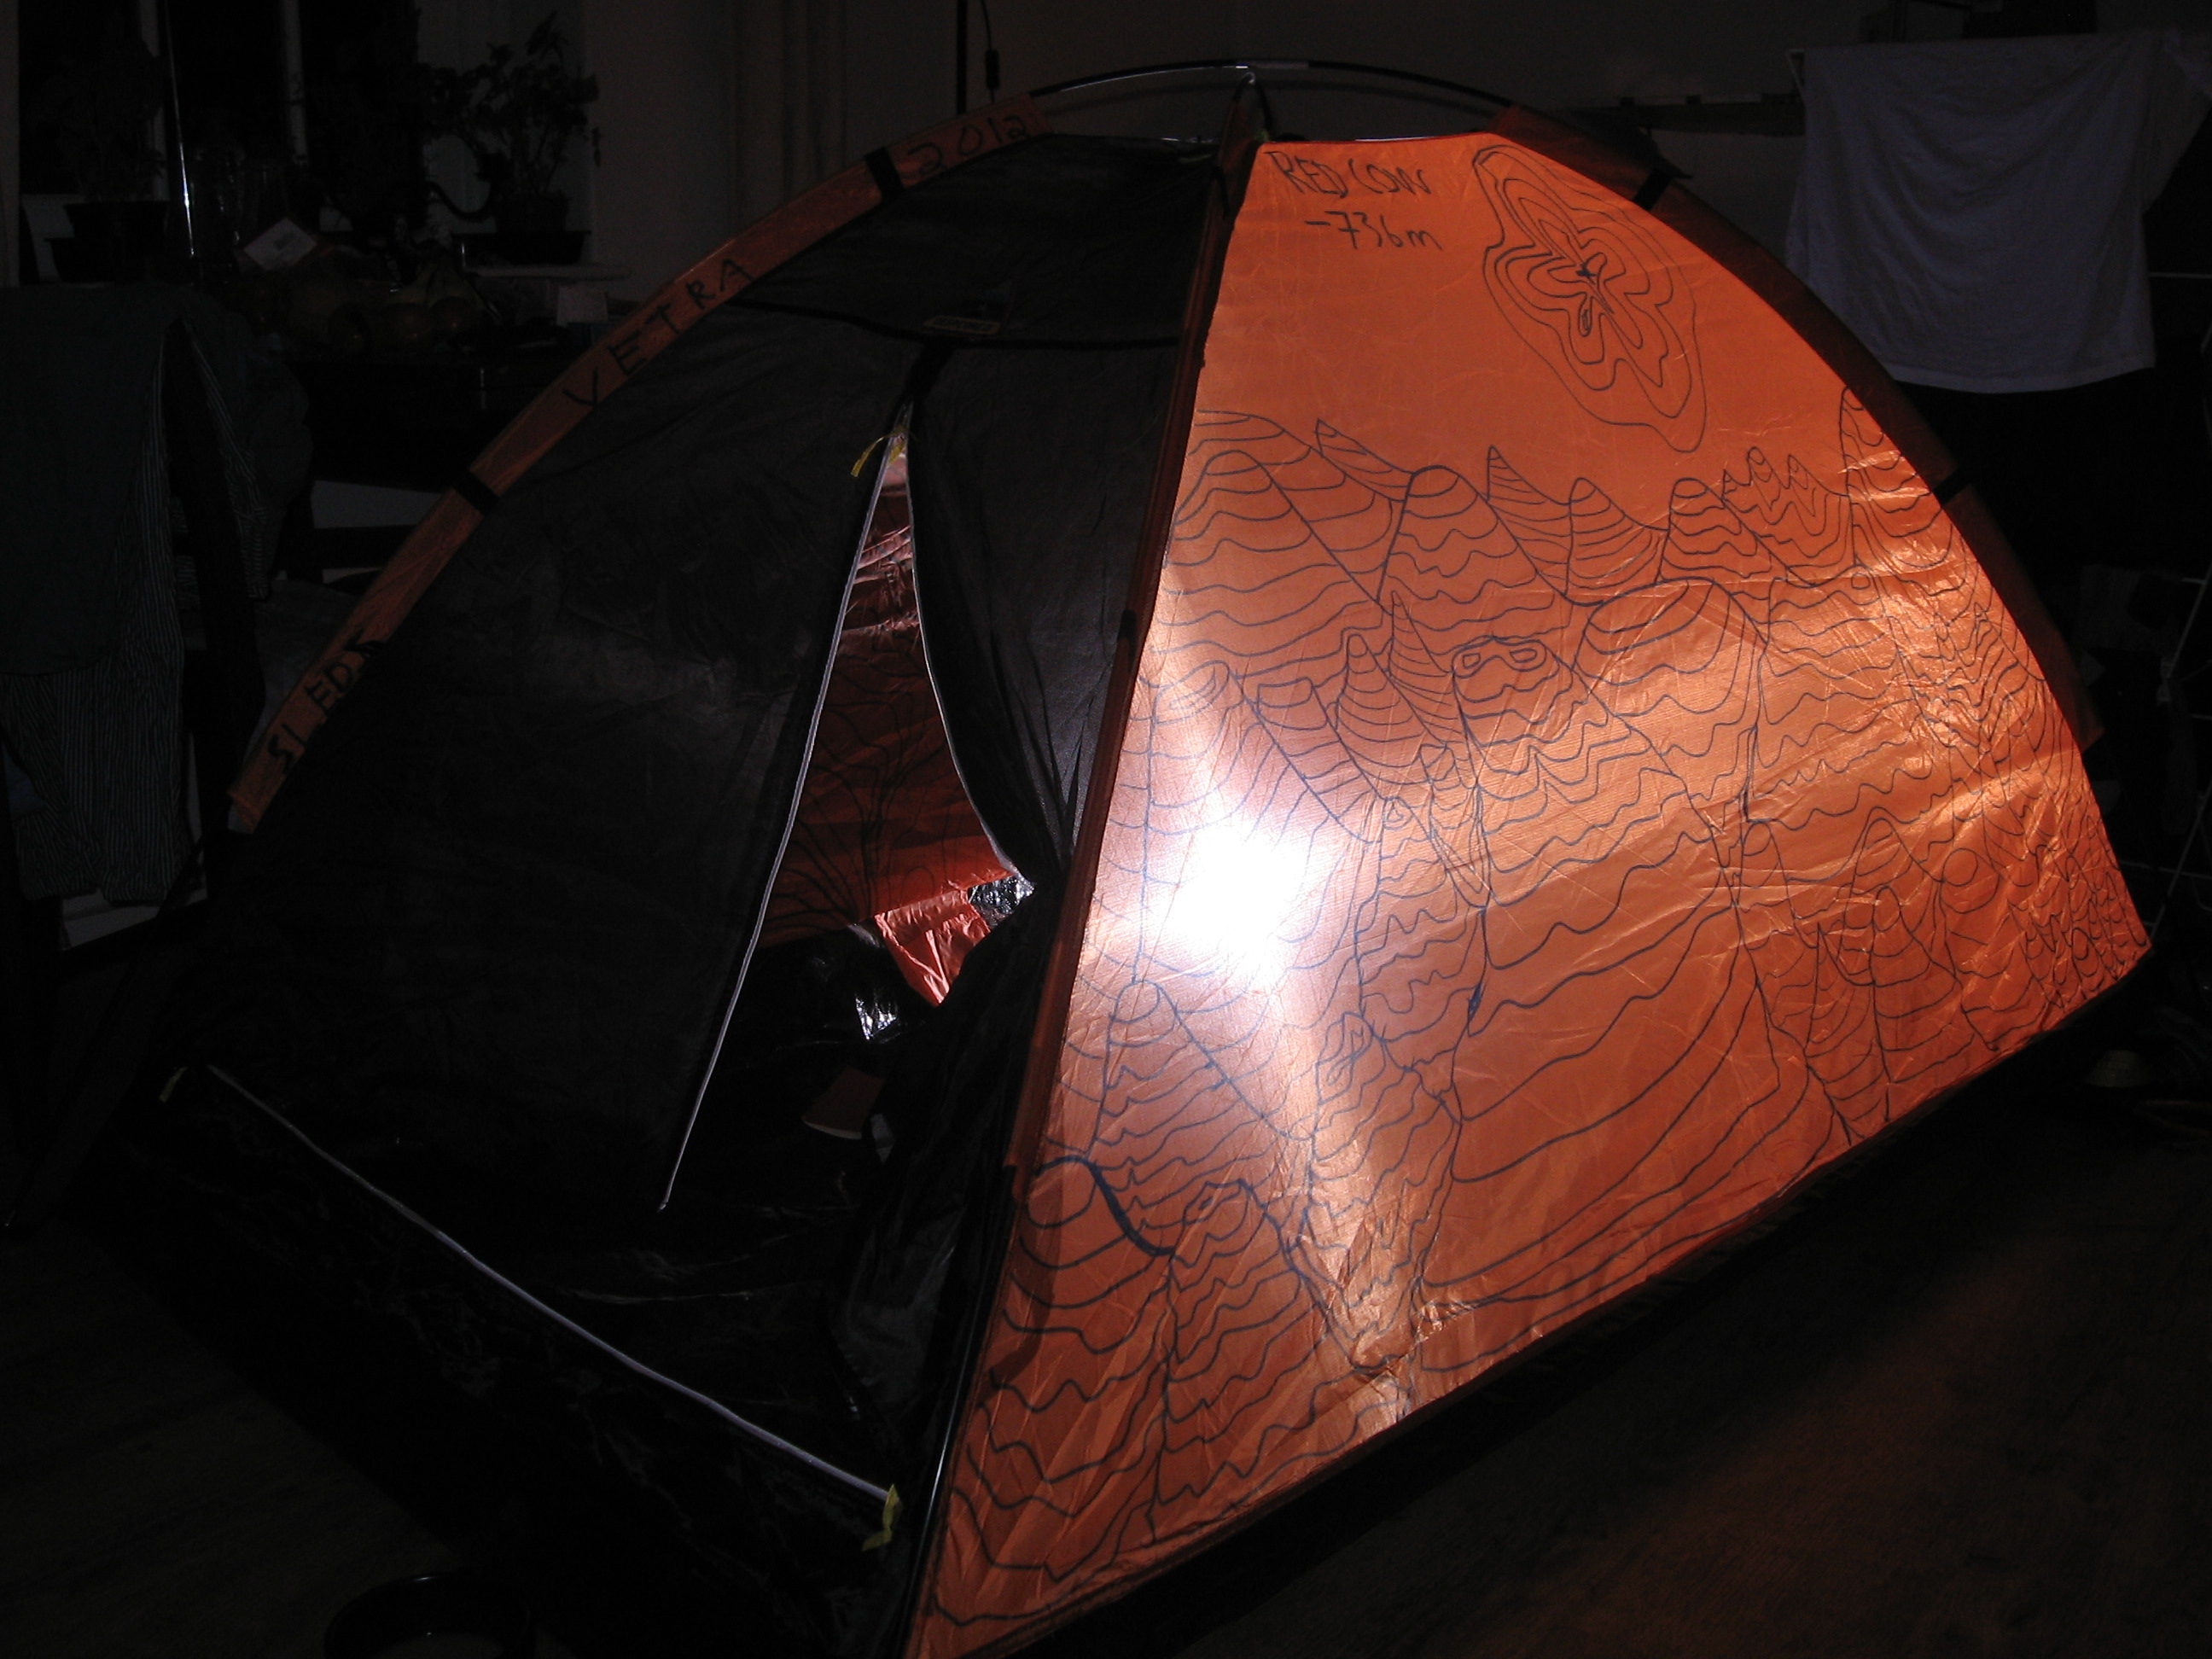
\includegraphics[width=\linewidth]{2012/diving_dreams/2012-07-12-JarvistMooreFrost-RedCowCampTent--orig.jpg}} 
 \caption{The tent readied for \passage{Red Cow Roundabout}, -736m \passage{Vrtnarija}. "What we lack in funding we make up for in leftfield art installations." \pic{Jarvist Frost}}
 \label{red cow tent}
\end{marginfigure}

Ideally the diving also required the setting up of a camp at \passage{Red Cow}. I
had prepared a lightweight two-man camp for this application, and had
assumed that people would at least be interested in visiting the bottom
of the cave or extending the leads further North in the deep levels.
However, one can't really direct exploration in this way, and the
majority of the expedition efforts went into the extensive horizontal
levels found below \passage{Stuck in Paradise} -- only two trips went
beyond \passage{Big Rock} this summer, and I was on both of them.

I solo'd my way to \passage{X-Ray} with a 7 Litre bottle and fin in a
tacklesac, and a weight belt of 8 kg of lead. This was actually found to
be not too difficult, though frightening on the little down climbs!

Approaching the end of my three weeks on the mountain, I finally had to
accept that the sumps were out of my reach. I was exhausted through my
efforts, making myself sick through not enough rest.

My last mad plan involving hijacking the ever eager Oli and spending
essentially three days portering gear to the dive site, diving, and
abandoning cylinders for the winter, was replaced by a rather more sane
plan to explore the bottom, and, sadly, drag my cylinder out from camp\sidenote{see overleaf}.

I pulled my shoulder really quite badly during this trip, which made my
slow exit from \passage{X-Ray} hauling steel arduous and painful. The
situation on the surface wasn't much more pleasant. The \passage{Bivi} talk was
full of suspicion that I would abandon without carrying all the dive
gear (and, indeed, my unused photographic gear) down. So there was
nothing to do but swipe opiates from the first aid kits, ignore my
grinding bones and do my carrying duty. I must admit it was with
considerable sadness and little will to return that I finally struck my
tent, squeezed the last few bits into my rucksack, ached down the
mountain and boarded a bus out of \passage[town]{Tolmin}.

My 8 kg of diving Lead sits at \passage{X-Ray} currently labelled with a
simple note:- ´Jarv's Folly¡

Everything is clear in hindsight. I should never have started preparing
to dive, instead put my efforts into dry exploration \& bolt climbing of
the deep levels and, potentially, readying the ground for a diving trip
in future years. Still, we live and learn, and ´Ah, but a man's reach
should exceed his grasp, or what's a Heaven for?´

\name{Jarvist Moore Frost}





\section{Watership Up with Oli}

Oli hadn't yet been on the serious pushing trip he was clearly capable
of. Having abandoned diving plans, I went down with him on the standard
two nighter. First stop, before bed, was the fabled \passage{Esoterica}. This was
quite an interesting place, being a streamway cutting through the \passage{Prince
Consort Road} horizontal level before the \passage{Albert Hall}. The \passage{Serpentine}
stream at the \passage{Albert Hall} almost certainly forms the development which
goes all the way to \passage{Watership Down}, there's every reason to
believe this streamway may proceed similarly. However, tales of wet rift
from the original explorers (James KP and Jan in 2010) have dissuaded a
return. We found the climb down through the boulders, and arrived at the
10 m pitch (taking water from the little inlet in the left of \passage{Prince
Consort Road}) I'd previously stood at. We commenced bolting, taking
turns.

\margininbox{Esoterica}{
     \begin{itemize}
    \item Jarvist Frost
    \item Oliver Myerscough
    \end{itemize}}{\explo}

While Oli was tapping away, I climbed over the rift pitch, down a 4
metre free climb and intersected a different stream. This stream came
down (on the left) from an easily gained chamber, with vast quantity of
beautiful haematite on the shelves. The continuation (to the right \&
following the stream down) was obvious, and I can only assume that this
is \passage{Esoterica} as pushed by James KP and Jan.

I related this to Oli back at the pitch head. We finished the backup
bolt no problem, but horror of horrors, broke the driver placing the
hang bolt. A few minutes experimenting with alternative natural rigging
(all too dodge) and we accepted unhappy defeat. Should have brought a
second driver. Should have brought the drill. I left a long and
meandering note underlining the point that this pitch was not dropped,
and the way to what I believe is \passage{Esoterica}.

It's one of those strange quirks of expedition -- we had what seemed to
be two independent streamways, both going and barely an hour away from
camp. Yet no one returned here either.

Having decided returning to camp for a replacement driver was too long a
round trip, I took Oli on a tourist trip to \passage{Palace of King Minos}.
We admired both the formations, the unpleasant nature of
`\passage{Guillotine}' and the admirable efforts in bolt climbing the
\passage{Queen's Bedchamber}, and returned via the \passage{Ouroboros} alternative to
the \passage{Albert Hall} -- odd passage formation indeed.


\subsection{Day 2}

We set off for the deep. I find \passage{Big Rock} a rather unfriendly place.
Though no one had been here since my previous trip (in 2011), I found a
lot of the bolts disturbingly loose. Always a worry with rawl bolts; I
also had dark thoughts of some kind of bolt loosening cave monster,
which I imagined as some kind of spanner assisted sloth.

The way to \passage{Red Cow} was almost second nature now -- the third time in two
years. I pointed out the few bits I'd figured out about the route on the
way, and dealt the stack of playing cards I had filled my Meander pocket
with (arrows and `\passage{Red Cow}' or `\passage{Big Rock}' to way-mark the two opposite
destinations). At \passage{Red Cow}, we repacked and left a Daren drum and food
stash, then continued on down to the bottom with a single bag of bolting
kit, rope and survey gear. Oli made short work of the sideways wriggles
in \passage{Winter Journey}, and with sanity rather than wanderlust on our
side we set about rigging the steep muddy climbs which Clare \& I had
slithered down and had such trouble climbing back to safely. While I merrily tapped in
the first bolt, Oli had a quick look at the `upwind' route from the
T-junction and came back shortly having wandered to the bottom of a
climb he didn't fancy by himself.

At the main climb, I realised I'd rigged the scrappy ropes we'd brought
in the wrong length order---Oli sorted this out behind me while I
placed a Y-hang off the opposite walls. The depth of the dry silt was
impressive---I chiseled off 5cm deep plates from both walls to find the
rock. (I suppose these are the result of the mostly static sump backing up - Tetley said that the sumps in SysMig were similar.)

Arriving at the sump with rather more poise and grace than last time, we
noted that the plastic PSS at the shore edge had floated off into the
sump -- clearly the level had increased (at least minutely) at some
point during the previous two weeks. I also threw a few rocks in the
sump to try and gauge how deep it was (4 m I estimate) and stomped in
the shallows a bit to try and assess the visibility for diving potential
(remarkably good, surprisingly no brown mud, the coarse sand settling
very quickly). Wearing my wet socks, I was trying to psyche myself up
into traversing along the right hand (sloping rock ledge) of the sump to
try and assess whether it continued around the corner, or stopped with a
rock wall.

\margininbox{Watership Up}{
     \begin{itemize}
    \item Jarvist Frost
    \item Oliver Myerscough
    \end{itemize}}{\explo}

Oli reckoned he could have a chance at the balcony, and prussic'd up the
rope before swinging across. He left the rope pulled over, but having
got together our survey instruments I grew bored of waiting for him to
return, and flicked the rope off to follow.

The level gained, \passage{Watership Up}, was really quite interesting -- very
difficult to tell how it formed, other than the obvious bedding plane
bit and with strange (large!) echoes leading off from tight rifts.
Following the natural route past puddles of Haematite and along a
protracted flat out squeeze we came to a section of rift with a drop
down onto a lake. This was a definite lake, as we could see both ends of
the body of water, but otherwise looked very similar to the main sump.
The pitch-head down from the rift would be narrow but certainly doable.
We surveyed our way back, notably there was a collection of those
strange spider-web like filaments covered with droplets in a cranny of
the rock. Always a bit spooky when you come across them -- no matter how
much one reminds oneself that they must be some kind of slime mould or
fungus, the image of a massive cave spider is hard to shake!

\tweet{10:05AM Aug 7, 2012}{WATERSHIPDOWN,climb made above lake at -900m,gaining continuation of inclined bedding plane to overlook another crystal clear still lake.}

With time already surprisingly tight, and a long way to climb, we set
off out, pulling all the ropes up with a bittersweet melancholy. We had
put the rigging effort in to further the next party, and effortlessly
found passage, but there remained so many question marks, and no other
parties intended to return down here this year.

Back at \passage{Red Cow} we toasted our mackerel with a splash of the meths
recovered from `\passage{Daydreamers}', and then had a warm Vitaminski (pusher's
delight). We filled up our Daren drum with water -- measuring the \passage{Red
Cow} stream as 1L/s (by filling a 6L Daren drum in a timed 10s, capturing
about 60\% of the stream). This Daren, along with the `bivi liberated'
mess tin and blue 2L Sigg bottle (with perhaps 200 ml of meths left) was
left sitting in the sand of the main \passage{Red Cow} passage. There was talk of
bolt climbers making their way down this way to investigate `\passage{Strap on
the Nitro}'. This didn't happen, and so those resources stand there
currently, awaiting the 2013 developments.

The slog on home to \passage{X-Ray} continued with little comment -- other
than I managed to pull a shoulder on the \passage{Memory Lane} climbs. We also
managed to flood the passage with smoke by leaving the fish tin to burn
itself out (thus burning the paint). Interestingly, and in contradiction
to the original explorers memories, the cave draft took this in the
direction of \passage{Big Rock}, we found ourselves caving through this fug till
at least \passage{Memory Lane}.

The way out from \passage{X-Ray}, with diving cylinder in tow, was slow
indeed. I sent Oli off ahead, and laboured my way behind. Some of the
\passage{Urinal series} pitch heads were really quite acrobatic when dragging a
third leg through!

\name{Jarvist Moore Frost}


